\documentclass[12pt]{article}
\usepackage{amsmath}
\usepackage{graphicx}
\usepackage{mathtools} %For summations with limits
\usepackage{multicol} %For multiple columns
\usepackage{comment} %So I don't have to put %'s in front of everything
\setlength{\columnsep}{1cm}

\begin{document}

\begin{titlepage}
    \begin{center}
	\vspace*{1cm}
 
	\Huge
	\textbf{Random Functions and Early Universe Cosmology}
 
	\vspace{0.5cm}
	\Large
 
	\vspace{1.5cm}
 
	Low Lerh Feng \\
	Student ID: 922910395
 
	\vfill
 
	Main supervisor: Richard Easther\\
	Co supervisor: Shaun Hendy
 
	\vspace{0.8cm}
 	Department of Physics, University of Auckland\\
	October 2018
    \end{center}
\end{titlepage}

\section{Aims and Objectives}

\begin{comment}

In the case of inflation, studies of stochastic inflation \re{cite Linde and others; early 90s and maybe before}  suggest that the same mechanism that produces astrophysical density perturbations could also support {\em eternal inflation\/} and the resultant generation of infinite numbers of  {\em pocket universes\/} \re{cite}. Likewise, the study of flux compactified string vacua points to the possible existence of a {\em landscape\/} \re{cite} or {\em discretuum\/} \re{cite}  of vacua within the theory. Conversely, the discovery that the vacuum energy is apparently non-zero (irrespective of whether it is also dynamical) opens the door to anthropic explanations of its value, insofar as a value that was apparently exactly zero could be suggestive of an underlying symmetry. 

 On its own, stochastic (or eternal) inflation  implies the existence of an apparent multiverse composed of many pocket universes, but not require that the ``low energy" (ie LHC scale) physics or vacuum  differs between pockets. For example in the quadratic inflation model is potentially eternal, but it has a unique vacuum.  However, landscape hypotheses posit the existence of multiple vacua which can, in principle, be populated by stochastic inflation. The best known of these is the string landscape itself, built on the plethora of flux-stablilsed vacua that exist inside Calabi-Yau spaces, but it is not necessarily a unique realisation of this scenario. The complexity of landscape itself and the vast number of vacua it provides is effectively part of its purported explanatory power � as the number of vacua is almost uncountably large (e.g. $10^{500}$ or greater \re{cite here}) it is conceivable that almost any value of the vacuum energy can be realised within it. 
 
 The detailed properties of any landscape are almost entirely unknown -- it is still far from clear whether any specific stringy construction  realises  the $SU(3) \times SU(2) \times U(1)$ gauge group of the Standard Model; more recently the Swampland Conjecture suggests that all stable minima of the theory might actually be ``underwater'' \re{cite}, or located at negative values of $\Lambda$ with the consequence that a positive dark energy contribution may in fact be due to a dynamical quintessence like evolution.   However, an alternative approach to understanding  landscape scenarios is to strip them down to their barest essence -- the proposal that multiverse cosmology is realised within a {\em random\/} multidimensional ($N\sim100$ or more) potential of interacting scalar fields. ``Random'' in this context is  in the sense of random function theory \cite{GRF1, GRF2, GRF3} whose properties often become more tightly defined as the dimensionality increases.\footnote{We refer to random functions not random fields, nomenclature often seen in the mathematical literature, to avoid confusion with the individual scalar fields that will be coupled by this potential.} In this approach  the apparent complexity of a multidimensional landscape will actually provide  leverage to that can be used to develop an understanding of its properties. 

\end{comment}

The theory of inflation is the current best explanation for certain perplexing observations of the Universe, such as the monopole problem, horizon problem, and flatness problem.\cite{Ryden} 
Inflation is thought to be caused by a scalar field. The simplest possibility is a one-dimensional scalar field analogous to the gravitational potential; however multidimensional scalar fields are also possible. In standard inflationary theory, the universe inflates when the gradient of the scalar field is small (so-called ``slow-roll inflation"), and stops inflating when we reach a minimum (a ``vacuum"). Early work on inflation led to the idea of \emph{eternal inflation}, whereby most of the universe inflates forever, but some patches reach local minima. These patches them become \emph{pocket universes}, each with its own laws of physics, one of which corresponds to our own. Of particular interest is that, if we are in one of these patches with a local minimum above zero, this ``vacuum energy" can manifest itself as a nonzero dark energy term -- and we observe dark energy. Hence, it is desirable to understand the nature of the scalar field behind inflation.

The precise nature of the scalar field behind inflation is unknown. However, the study of flux-compactified string vacua predicts the existence of a highly complex, $O(100)$ dimensional scalar field known as the \emph{landscape}. This landscape contains a vast number of vacua which can, in principle, be the scalar field of inflation. The main objective of this research is to map, given the landscape, the probability that we are in a minimum with vacuum energy equal to what we observe as a function of the number of dimensions $N$ in the landscape. 

There are two ways to attack the problem. The first is to try to understand the string landscape better, and derive a probability from first principles. The other is to ignore the theory that goes into the landscape and simply treat it as a statistical aggregate invoking the central limit theorem. The string landscape is astonishingly complex -- an often-quoted estimate of the number of vacua is $10^{500}$\cite{Douglas} -- and therefore, most studies of the landscape take the latter approach.\cite{GRF1, GRF2, GRF3} We assume the landscape is well-approximated by a Gaussian random field, and try to determine the probability of a minimum with a value equal to the one we measure.

\section{Contribution}
By definition, Gaussian Random Fields have set correlations between its field value, first derivative, and second derivative at every point. For example, the first derivative and second derivative of a Gaussian Random Field are completely uncorrelated. They are generic constructs not specific to cosmology, and their properties have been widely studied. One early paper dealt with the relative abundances of maxima, minima, and saddles.\cite{Aazami2006} The authors took the Hessian of a random function to be symmetric matrices with random individual elements, or more precisely, with values randomly drawn from a Gaussian distribution (called a Gaussian Orthogonal Ensemble [GOE]). From elementary calculus, a minimum exists if the eigenvalues of the Hessian are all positive, a maximum exists if they are all negative, and there is a saddle if there are eigenvalues of both signs. Using the GOE, they find that the number of minima is super-exponentially small compared to the number of saddles. This approach was later shown to be incorrect, because the eigenvalues of the Hessian of a random function are not independent of each other \cite{Easther2016}. Taking this into account, the authors found that the number of minima decreases exponentially with the number of dimensions $N$ instead, and the ratio of extrema to saddles to be approximately binomial.

In addition to the probability of minima, the distribution of eigenvalues of the Hessian about minima as well as the distribution of the Hessian itself as a function of $N$ has also been investigated.\cite{Yamada2018}\cite{Fyodorov2018} Yamada and Vilenkin\cite{Yamada2018} found that in a Gaussian random landscape the smallest eigenvalue is of order $\sim 1/N$, which, if one assumes that the most probable decay pathway is in the direction of the smallest eigenvalues, improves the stability of the minima by about $\sqrt{N}$.

Aside from the properties of the field itself, questions such as the probability of moving from a random point in the potential to a viable late-time de Sitter minimum by Dyson Brownian motion have also been asked.\cite{Pedro2017} Pedro and Westphal calculated the probability of a graceful exit from random points in the landscape, and found that there is an exponential bias against small-field inflationary ranges, which allows us to conclude that the observation that the universe is flat imposes a $N \ll 10$ constraint on the number of light fields involved in inflation.

None of these works, however, have explicitly examined the probability that a field point of known value is a minimum or maximum (Bardeen et al\cite{BBKS} touched on it while dealing with a different problem on the number density of stationary points). So far in this project, we have explicitly generalized Bardeen et al's (henceforth BBKS) calculation from 3-dimensions to $N$-dimensions, reaching a maximum of $N=10$.

\section{Preliminary results}
The final probability depends not only on the field value $\phi$ but also the moments of the power spectrum $\sigma_0, \sigma_1, \sigma_2$. That the probability depends on the intrinsic properties of the field is intuitively obvious, since a very turbulent random field will have a lot of minima and maxima, naturally pushing the probability to $\sim$0.5. It turns out that two of the three $\sigma$'s are normalizable. $\sigma_0$ is closely related to the average value of the field, so with an appropriate choice of the zero of the field, we can set $\sigma_0 = 1$. Similarly, $\sigma_1$ represents the average of the first derivatives, and with an appropriate rescaling of the axis length we can also set it $\sigma_1 = 1$. This leaves $\sigma_2$ as the only remaining parameter, and all the results we present will be in terms of $\sigma_2$.

\begin{figure}
  \centering
  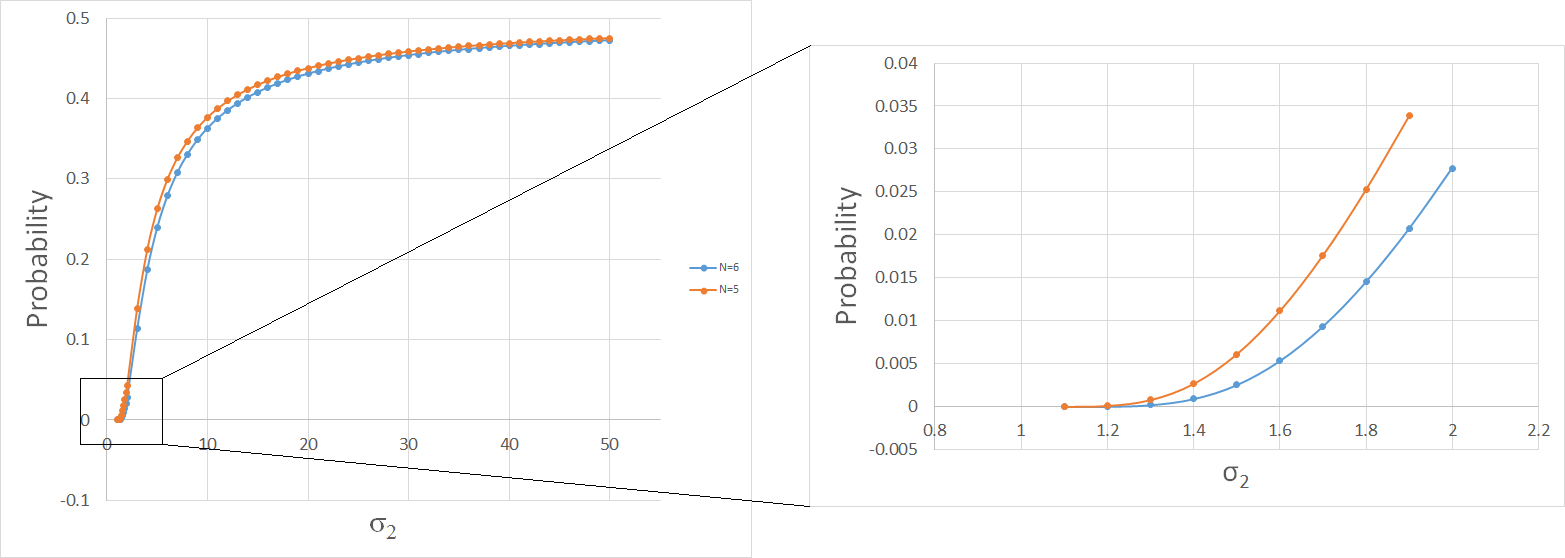
\includegraphics[width=\linewidth]{N6minima.png}
  \caption{The probability that a given extremum with $\phi > 0$ is a minimum as a function of $\sigma_2$, for $N=5,6$. A close-up of the probabilities for small values of $\sigma_2$ is shown as well. The probability for $N=5$ is always larger than that for $N=6$.}
  \label{N6}
\end{figure}

We performed analytical calculations up to $N=6$. The results are given in Fig. \ref{N6}. Here we plot the probability that a given extremum with $\phi > 0$ is a minimum as a function of $\sigma_2$. As expected, if the potential is highly oscillatory (i.e. $\sigma_2$ is large, or $\gamma$ is small), the probability tends towards 0.5 -- equal likelihood of an extremum being either a maximum or a minimum. Conversely, if the potential is very smooth ($\sigma_2$ is small), the probability tends towards 0. Further, for any given $\sigma_2$, the probability decreases with increasing dimension.

For $N > 6$, the calculations are complex enough that we have to attack the problem numerically. This works up to $N=10$. The results are given in Table 1. The same trends are seen: for any given $\sigma_2$, the probability decreases with increasing dimension.

\begin{table}[h!]
  \begin{center}
    \caption{The probability that a given extremum with $\phi > 0$ is a minimum as a function of $\sigma_2$. Values given for $N=4,5,6$ are exact; for larger values they are approximate (see the text; errors are on the order of the third nonzero digit after the decimal).}
    \label{tab:table1}
    \begin{tabular}{c|c|c} % <-- Alignments: center/center/center (l and r for left and right if needed)
      $\textbf{N}$ & $\sigma_2$ & $p_{min}$\\
      \hline
      4 & 10 & 0.60859\\
      5 & 10 & 0.62333\\
      6 & 10 & 0.63680\\
      7 & 10 & 0.35210\\
      8 & 10 & 0.34227\\
      9 & 10 & 0.33159\\
      10 & 10 & 0.32151\\
      \hline
      4 & 3.5 & 0.21520\\
      5 & 3.5 & 0.17886\\
      6 & 3.5 & 0.15274\\
      7 & 3.5 & 0.13599\\
      8 & 3.5 & 0.11711\\
      9 & 3.5 & 0.10093\\
      10 & 3.5 & 0.08729\\
      \end{tabular}
      \quad
      \begin{tabular}{c|c|c} 
      $\textbf{N}$ & $\sigma_2$ & $p_{min}$\\
      \hline
      4 & 2 & 0.066638\\
      5 & 2 & 0.043103\\
      6 & 2 & 0.030844\\
      7 & 2 & 0.02013\\
      8 & 2 & 0.01307\\
      9 & 2 & 0.00845\\
      10 & 2 & 0.00544\\
      \hline
      4 & 1.25 & 0.001526\\
      5 & 1.25 & 0.000327\\
      6 & 1.25 & 6.53328 $\times 10^{-5}$\\
      7 & 1.25 & 2.09673 $\times 10^{-5}$ \\
      8 & 1.25 & 3.97235  $\times 10^{-6}$ \\
      9 & 1.25 & 7.13489  $\times 10^{-7}$ \\
      10 & 1.25 & 1.20253  $\times 10^{-7}$ \\
     \end{tabular}
  \end{center}
\end{table}

\begin{figure} 
  \centering
  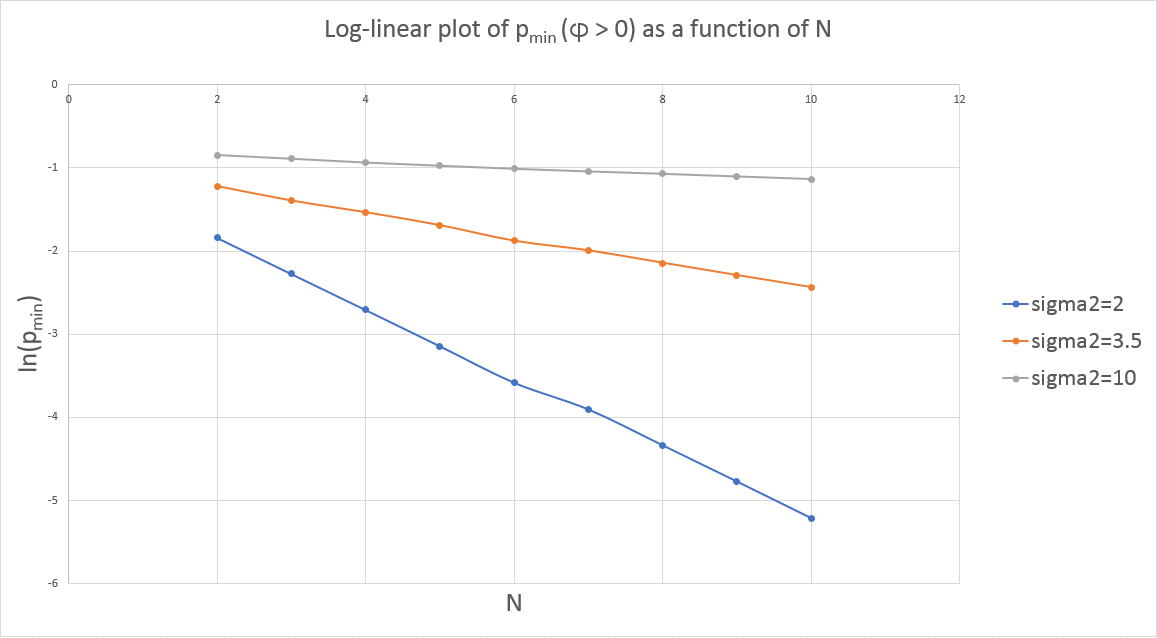
\includegraphics[width=\linewidth]{Log-linear.png}
  \caption{A log-linear plot of the probability that a given extremum with $\phi > 0$ is a minimum for a given $\sigma_2$, as a function of the number of dimensions $N$.}
  \label{Log-Linear}
\end{figure}

\section{Next steps}
Next up on the agenda is to investigate the behaviour of the field around saddles. These are stationary points which are not maxima or minima -- they increase in some directions and decrease in others. We do this because this is where inflation occurs. In standard inflationary theory, slow-roll inflation occurs when:

\begin{equation}
	\begin{split}
	\epsilon \equiv \frac{m_{Pl}^2}{2}\bigg(\frac{V'}{V}\bigg)^2 \ll 1
	\qquad
	|\eta| \equiv m_{Pl}^2 \frac{|V''|}{V} \ll 1
	\end{split}
\end{equation}

Here $m_{Pl}$ is the Planck mass. It's relatively easy to find points where $\epsilon \ll 1$ -- that will naturally happen about a maximum or minimum since $V'=0$ at those points, and we already know extrema exist. Not so easy is to find points where $\epsilon \ll 1$ \emph{and} $\eta \ll 1$. If our universe had inflated in the vicinity of these points, then it would have inflated for a varying amount (known as the number of e-folds of inflation) that depends on the value of $\eta$. We need 40--60 e-folds of inflation to solve the cosmological problems inflation was created to solve, \cite{Baumann} so we want to know $P(\eta)$ given that we need 40--60 e-folds of inflation. This compares to the already-accomplished work, where we solve for $P(\Lambda)$ given that we observe dark energy in the present universe.

Another thing we will investigate is how likely our universe is given that we observe a scalar spectral index $n_s$ of about 0.96 \cite{Planck}. This observable parameter is related to the slow-roll parameters via $n_s = -2\epsilon + 6\eta$, and acts as another link between our work and observations.

Note both $\epsilon$ and $\eta$ depend on the potential, its gradient, and its second derivative. These are things which the previous analysis equips us to analyze (they are after all intimately related to the $\sigma$'s).

\begin{comment}
\section{Methodology}
The main method used in this work is a generalization of the method used in Refs. \cite{Easther2016} and \cite{Masoumi2016}. After we had already reached $N=10$, we discovered that BBKS had derived an equation that can be easily adapted to our problem; we verified that the two methods give the same result. The two methods are technical and difficult to describe without two pages of equations. I will attempt it anyway, and refer the reader to the references for full details.

The number of minima in a region is:

\begin{equation}
N_{min}=\int d^Nx \delta^N (\phi,_i) |\mathrm{det}(\phi,_{ij})|\theta_H(\lambda_N)
\end{equation}

\noindent Here the commas represent derivatives, $i, j$ correspond to the spatial dimensions, $\theta_H$ is the Heaviside delta function, and $\lambda_N$ is the smallest eigenvalue of the Hessian matrix. The $\delta$-function imposes the condition that the first derivative is zero. The determinant term is the Jacobian arising from a change of variables of the expression within the delta function (notice the integral is over position, not over the gradient of the field). The Heaviside function imposes the condition that $\lambda_N \geq 0$, i.e. that all eigenvalues of the Hessian are positive. From elementary calculus, this is the statement that the point is a minimum.

Next we need the correlations of the field value, first derivatives, and second derivatives for Gaussian random fields. These are, by definition,

\begin{equation}
\begin{split}
\langle\phi\phi\rangle &= \sigma_0^2 \\
\langle\eta_i\eta_j\rangle &= \frac{1}{N}\delta_{ij}\sigma_1^2 \\
\langle\phi\eta_{ij}\rangle &= -\frac{1}{N}\delta_{ij}\sigma_1^2 \\
\langle\xi_{ij}\xi_{kl}\rangle &= \frac{1}{N(N+2)}\sigma_2^2(\delta_{ij}\delta_{kl}+\delta_{il}\delta_{jk}+\delta_{ik}\delta_{jl})
\end{split}
\end{equation}

\noindent where $\phi$ is the field value, $\eta_i$ is the first derivative in the $i$ direction, the $\sigma$'s are moments of the power spectrum, and $\xi_{ij}$ is the second derivative w.r.t. $i$ and $j$. To calculate the number of stationary points, we define the vector $\alpha$:

\begin{equation}
\begin{split}
\alpha_i = \{\phi,\eta_1,\eta_2,\ldots,\xi_{11},\xi_{22},\ldots,\xi_{NN},\xi_{N-1,N},\xi_{N-2,N},\ldots,\xi_{1N},\xi_{N-2,N-1},\\
\ldots\xi_{1,N-1},\ldots,\xi_{12}\}
\end{split}
\end{equation}

We define the covariance matrix $M_{ij}\equiv\langle\alpha_i\alpha_j\rangle$ and its inverse $K \equiv M^{-1}$. The probability distribution of $\alpha$ is (by definition for Gaussian random fields)

\begin{equation} \label{ProbDistrib}
p(\alpha_i)=\frac{1}{(2\pi)^{N(N+3)/4}\sqrt{\mathrm{det}M}} e^{-\frac{1}{2}\alpha K \alpha}
\end{equation}

The number of stationary points is then

\begin{equation} \label{NFormula}
N = \int d^Nx d \alpha_1 \ldots d\alpha_{N(N+3)/2} \delta^N(\eta_i) \mathrm{det}(\xi_{ij})\theta_H(\lambda)p(\alpha)
\end{equation}

We can transform the Hessian matrix into a function of its eigenvalues $\lambda$ and Euler angles, and change variables such that the integration limit is w.r.t the eigenvalues instead. For full details see the references. The final expression we arrive at for the density of peaks is:

\begin{equation} \label{DensityOfPeaks}
N = A \int_{\lambda_1 \geq \lambda_2 \geq \lambda_3 \ldots \geq 0} F \times e^{-\alpha K \alpha} d\nu dx dy dz \ldots
\end{equation}

\noindent where

\begin{equation}
F = \lambda_1\lambda_2\lambda_3\ldots\lambda_N \sum^N_{i,j; i>j} (\lambda_i - \lambda_j),
\end{equation}

\noindent $A$ is some constant factor (this cancels because we're interested in the probability, and both the denominator and numerator have factors of $A$), and the integration limits are only over the region where the conditions are satisfied. The rest of the project is ``just" evaluating this integral.
\end{comment}

\section{Ethical approval}
Not needed.

\section{Resources}
To perform the calculations, we need computational power and \emph{Mathematica}. Both of these we already have. If we turn out to need more computational power than a standard machine can provide, we also have access to the Nectar Cloud.

\section{Thesis structure}
I intend the thesis to be focused on work to be published over the next two years, which will focus on this topic and possibly others.

\begin{itemize}
\item Introduction
\begin{itemize}
\item Gaussian random fields
\item The string landscape and why approximating the landscape as Gaussian random fields makes sense
\item How inflation is related to the structure of the landscape
\end{itemize}
\item Theory
\begin{itemize}
\item A first-principles derivation of the theory required to make educated statements about the landscape's properties
\item Will involve a \emph{lot} of equations
\end{itemize}
\item Results
\begin{itemize}
\item Summary of the papers that will arise from this work
\item Probability of minimum at a known field value given that an extremum is there
\item Statements about the slow-roll parameters $\epsilon$ and especially $\eta$, and the implications these have on the number of e-folds of inflation we can expect as well as the scalar spectral index $n_s$
\end{itemize}
\item Conclusions
\end{itemize}

\section{Proposed timeline}
\begin{itemize}
\item Immediately or in the next two months: finish and submit the paper on the probability of minimum at a known field value given that an extremum is there.
\item Now--March 2019: Investigate the properties of $\epsilon$ and $\eta$ in the landscape. If possible extend these results as well as the previous one to even higher dimensions than $N=10$.
\item April 2019--October 2019: Connect these properties to observables. Publish these results.
\item November 2019--June 2020: Potentially we will change directions completely to a different subfield in cosmology; if not, continue to develop these results. For example we could ask how far saddles are from one another, and whether it's likely that the universe will undergo two separate periods of inflation.
\item June 2020--September 2020: Write up and defend thesis.
\end{itemize}

\begin{thebibliography}{99}
\bibitem{Ryden} B. Ryden, \emph{Introduction to Cosmology}, Cambridge University Press, 2003
\bibitem{GRF1} A. Masoumi, A. Vilenkin and M. Yamada, Journal of Cosmology and Astroparticle Physics, 05:053, 2017
\bibitem{GRF2} A. Masoumi, A. Vilenkin and M. Yamada, Journal of Cosmology and Astroparticle Physics, 12:035, 2017
\bibitem{GRF3} T. Bjorkmo and M.C.D. Marsh, Journal of Cosmology and Astroparticle Physics, 02:037, 2018
\bibitem{Aazami2006} A. Aazami and R. Easther, Journal of Cosmology and Astroparticle Physics (0603:013), 2006
\bibitem{Easther2016} R. Easther, A. Guth and A. Masoumi, arXiv:1612.05224 (2016)
\bibitem{Yamada2018} M. Yamada and A. Vilenkin. Journal of High Energy Physics 2018: 29, 2018
\bibitem{Fyodorov2018} Y. Fyodorov and P. Le Dossal, arXiv:1806.05294 (2018)
\bibitem{Pedro2017} F.G. Pedro and A. Westphal, A. Journal of High Energy Physics, 163, 2017
\bibitem{BBKS} J. M. Bardeen, J. R. Bond, N. Kaiser, and A. S. Szalay, Astrophysical Journal, Astrophysical Journal, vol. 304, page 15-61 (1986)
\bibitem{Masoumi2016} A. Masoumi, \emph{Statistics of stationary points in a landscape}, unpublished
\bibitem{Baumann} D. Baumann, \emph{The Physics of Inflation}, http://www.damtp.cam.ac.uk/user/db275/TEACHING/INFLATION/Lectures.pdf
\bibitem{Planck} Planck Collaboration, Planck 2018 results. VI. Cosmological parameters, arXiv:1807.06209 (2018)
\bibitem{Douglas} M. R. Douglas, Journal of High Energy Physics, 05:046, 2003
\end{thebibliography}

\end{document}